\subsection{Recipe}

In this section the recipe screen is going to be described. Both the functionality of the screen as well as the design priciples used in the design process is going to be described. The sketch used to illustrate the use consist of 2 different screens, one screen only showing a full screen of the recipe, and one screen showing how to browse through the recipe. The browsing screen is divided into 2 sketches, showing the functionality of this screen.

The images sketches refereed to can be seen in figure \ref{FinalRecipeBrowsingSketch1} and in figure \ref{FinalRecipeBrowsingSketch2}. The sketch in figure \ref{FinalRecipeBrowsingSketch1} is the first screen to see, when browsing recipes. The right screen in figure \ref{FinalRecipeBrowsingSketch2} show the expanded version of the recipe browsing screen, and the left shows the full screen of the recipe.

\begin{figure}[H]
    \centering
    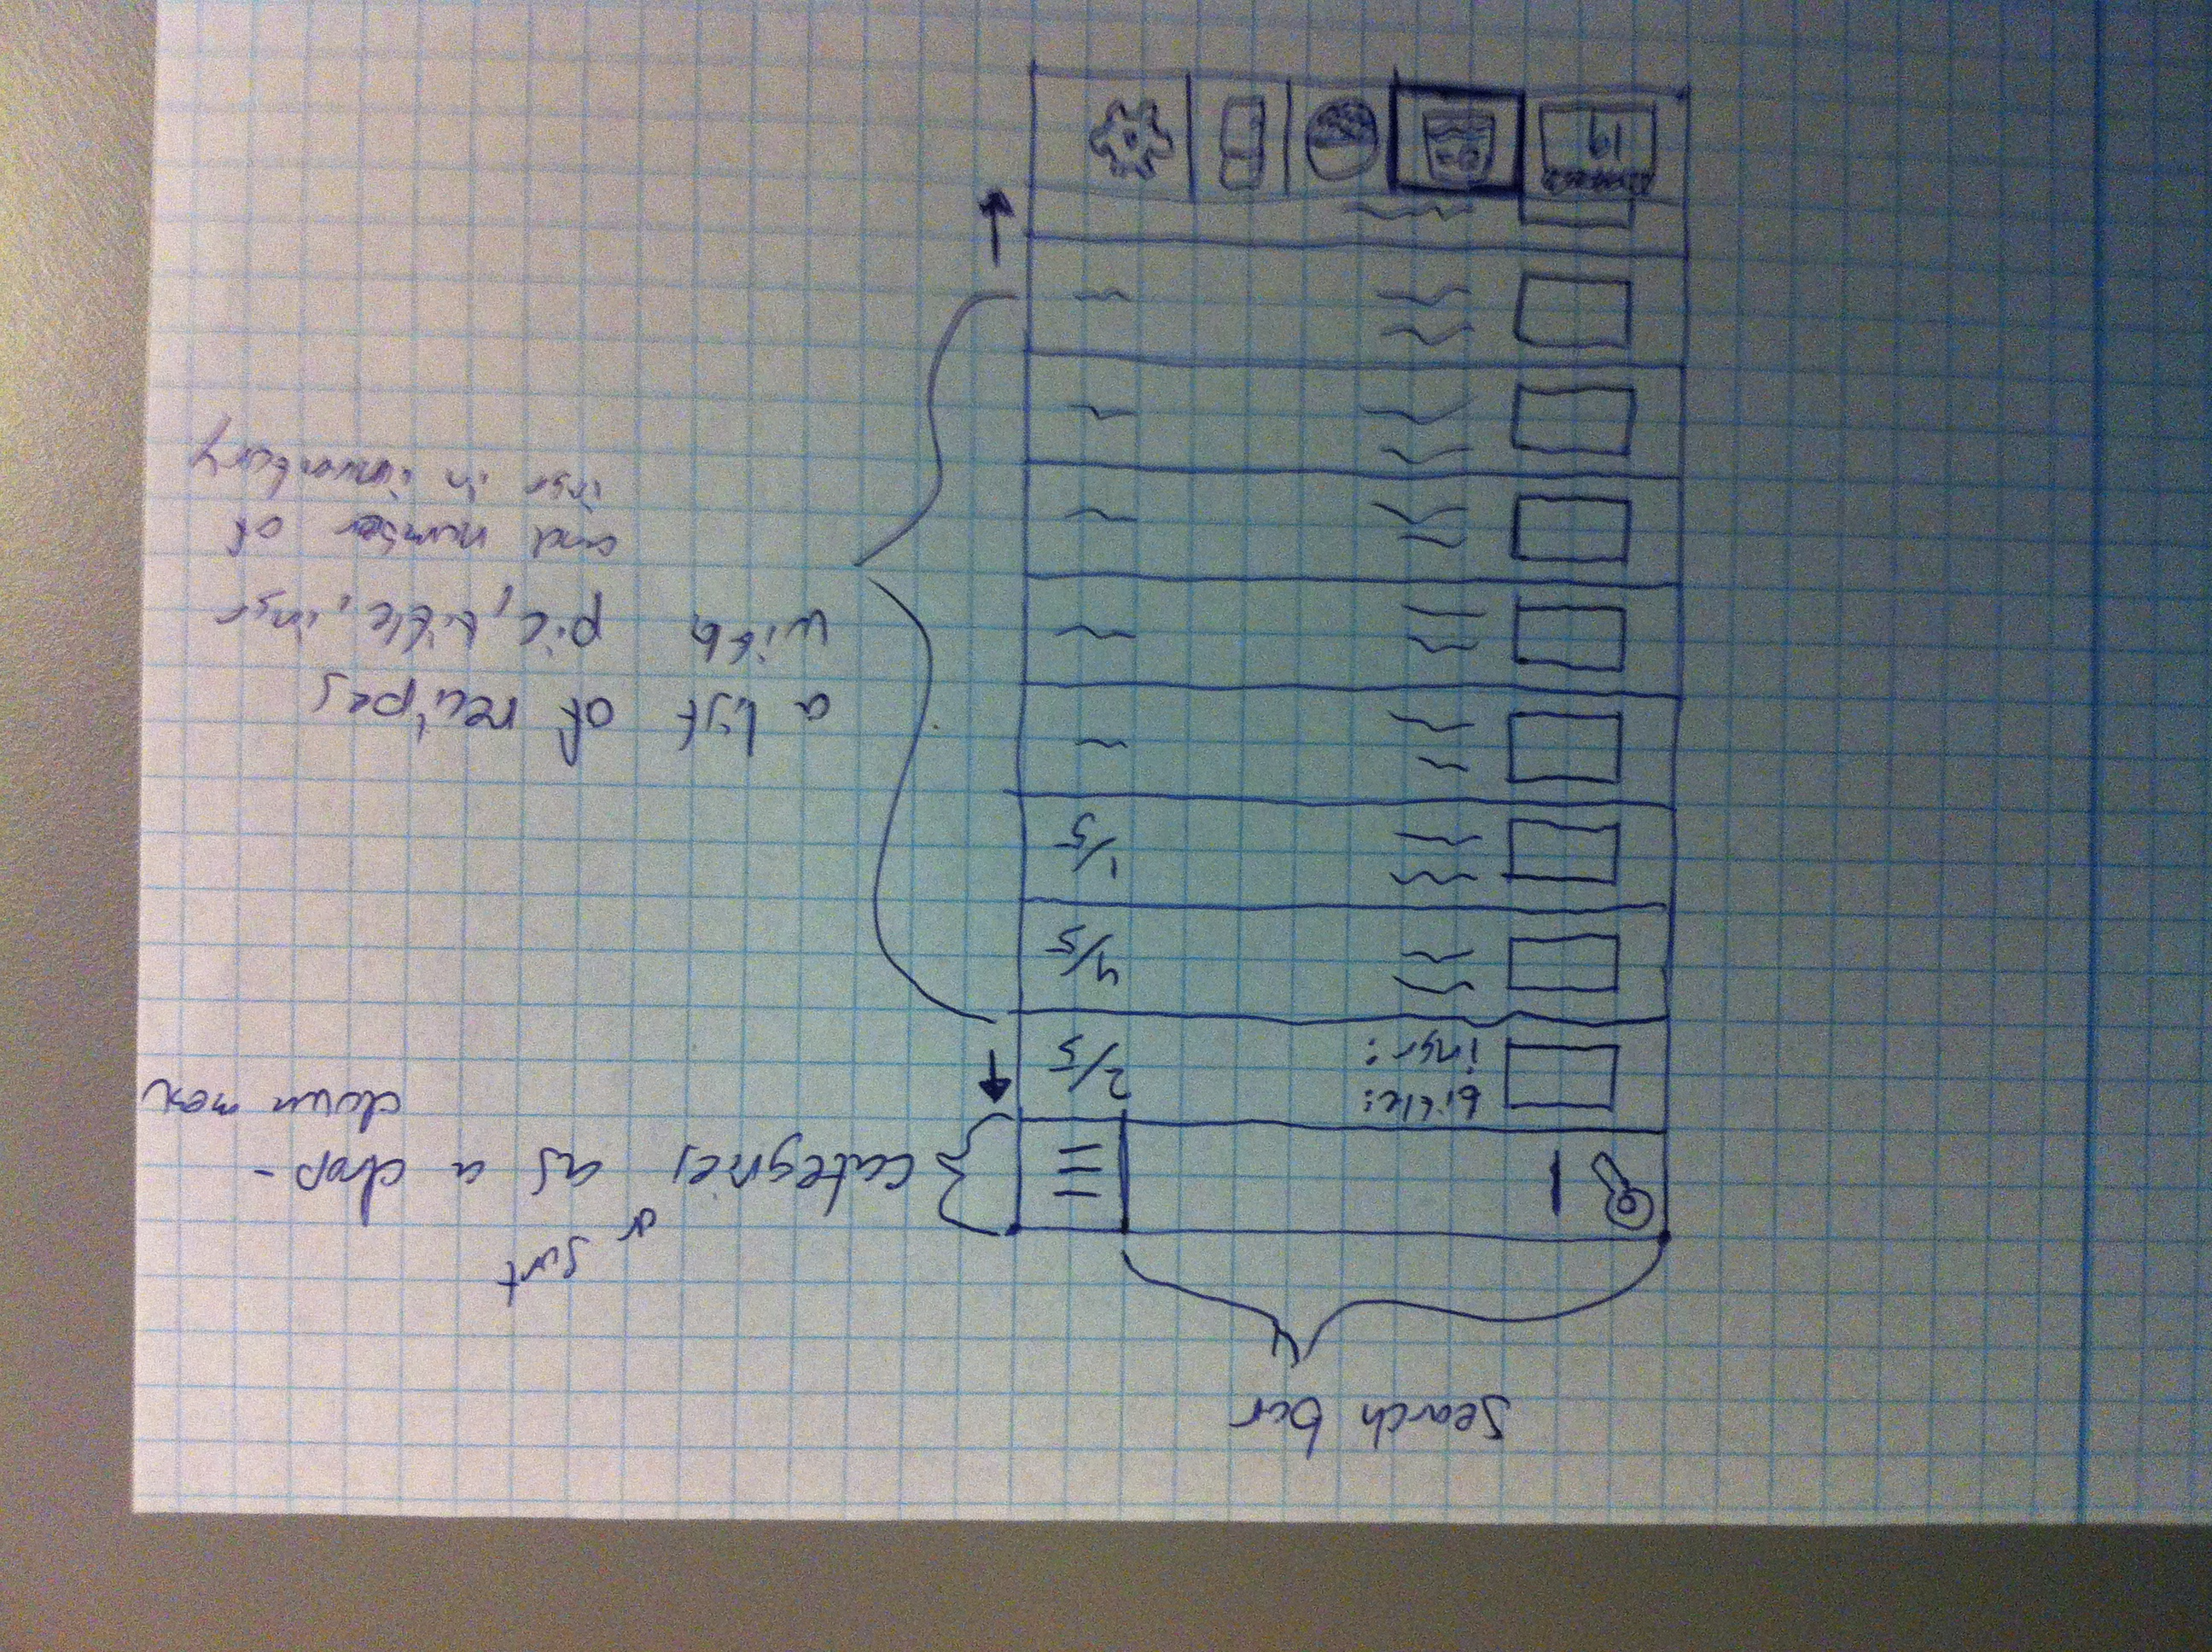
\includegraphics[width=0.5\textwidth]{Grafik/FoodPlanner/FinalRecipeBrowsingSketch1}
    \caption{One of the final sketch of the recipe browsing screen}
    \label{FinalRecipeBrowsingSketch1}
\end{figure}

\begin{figure}[H]
    \centering
    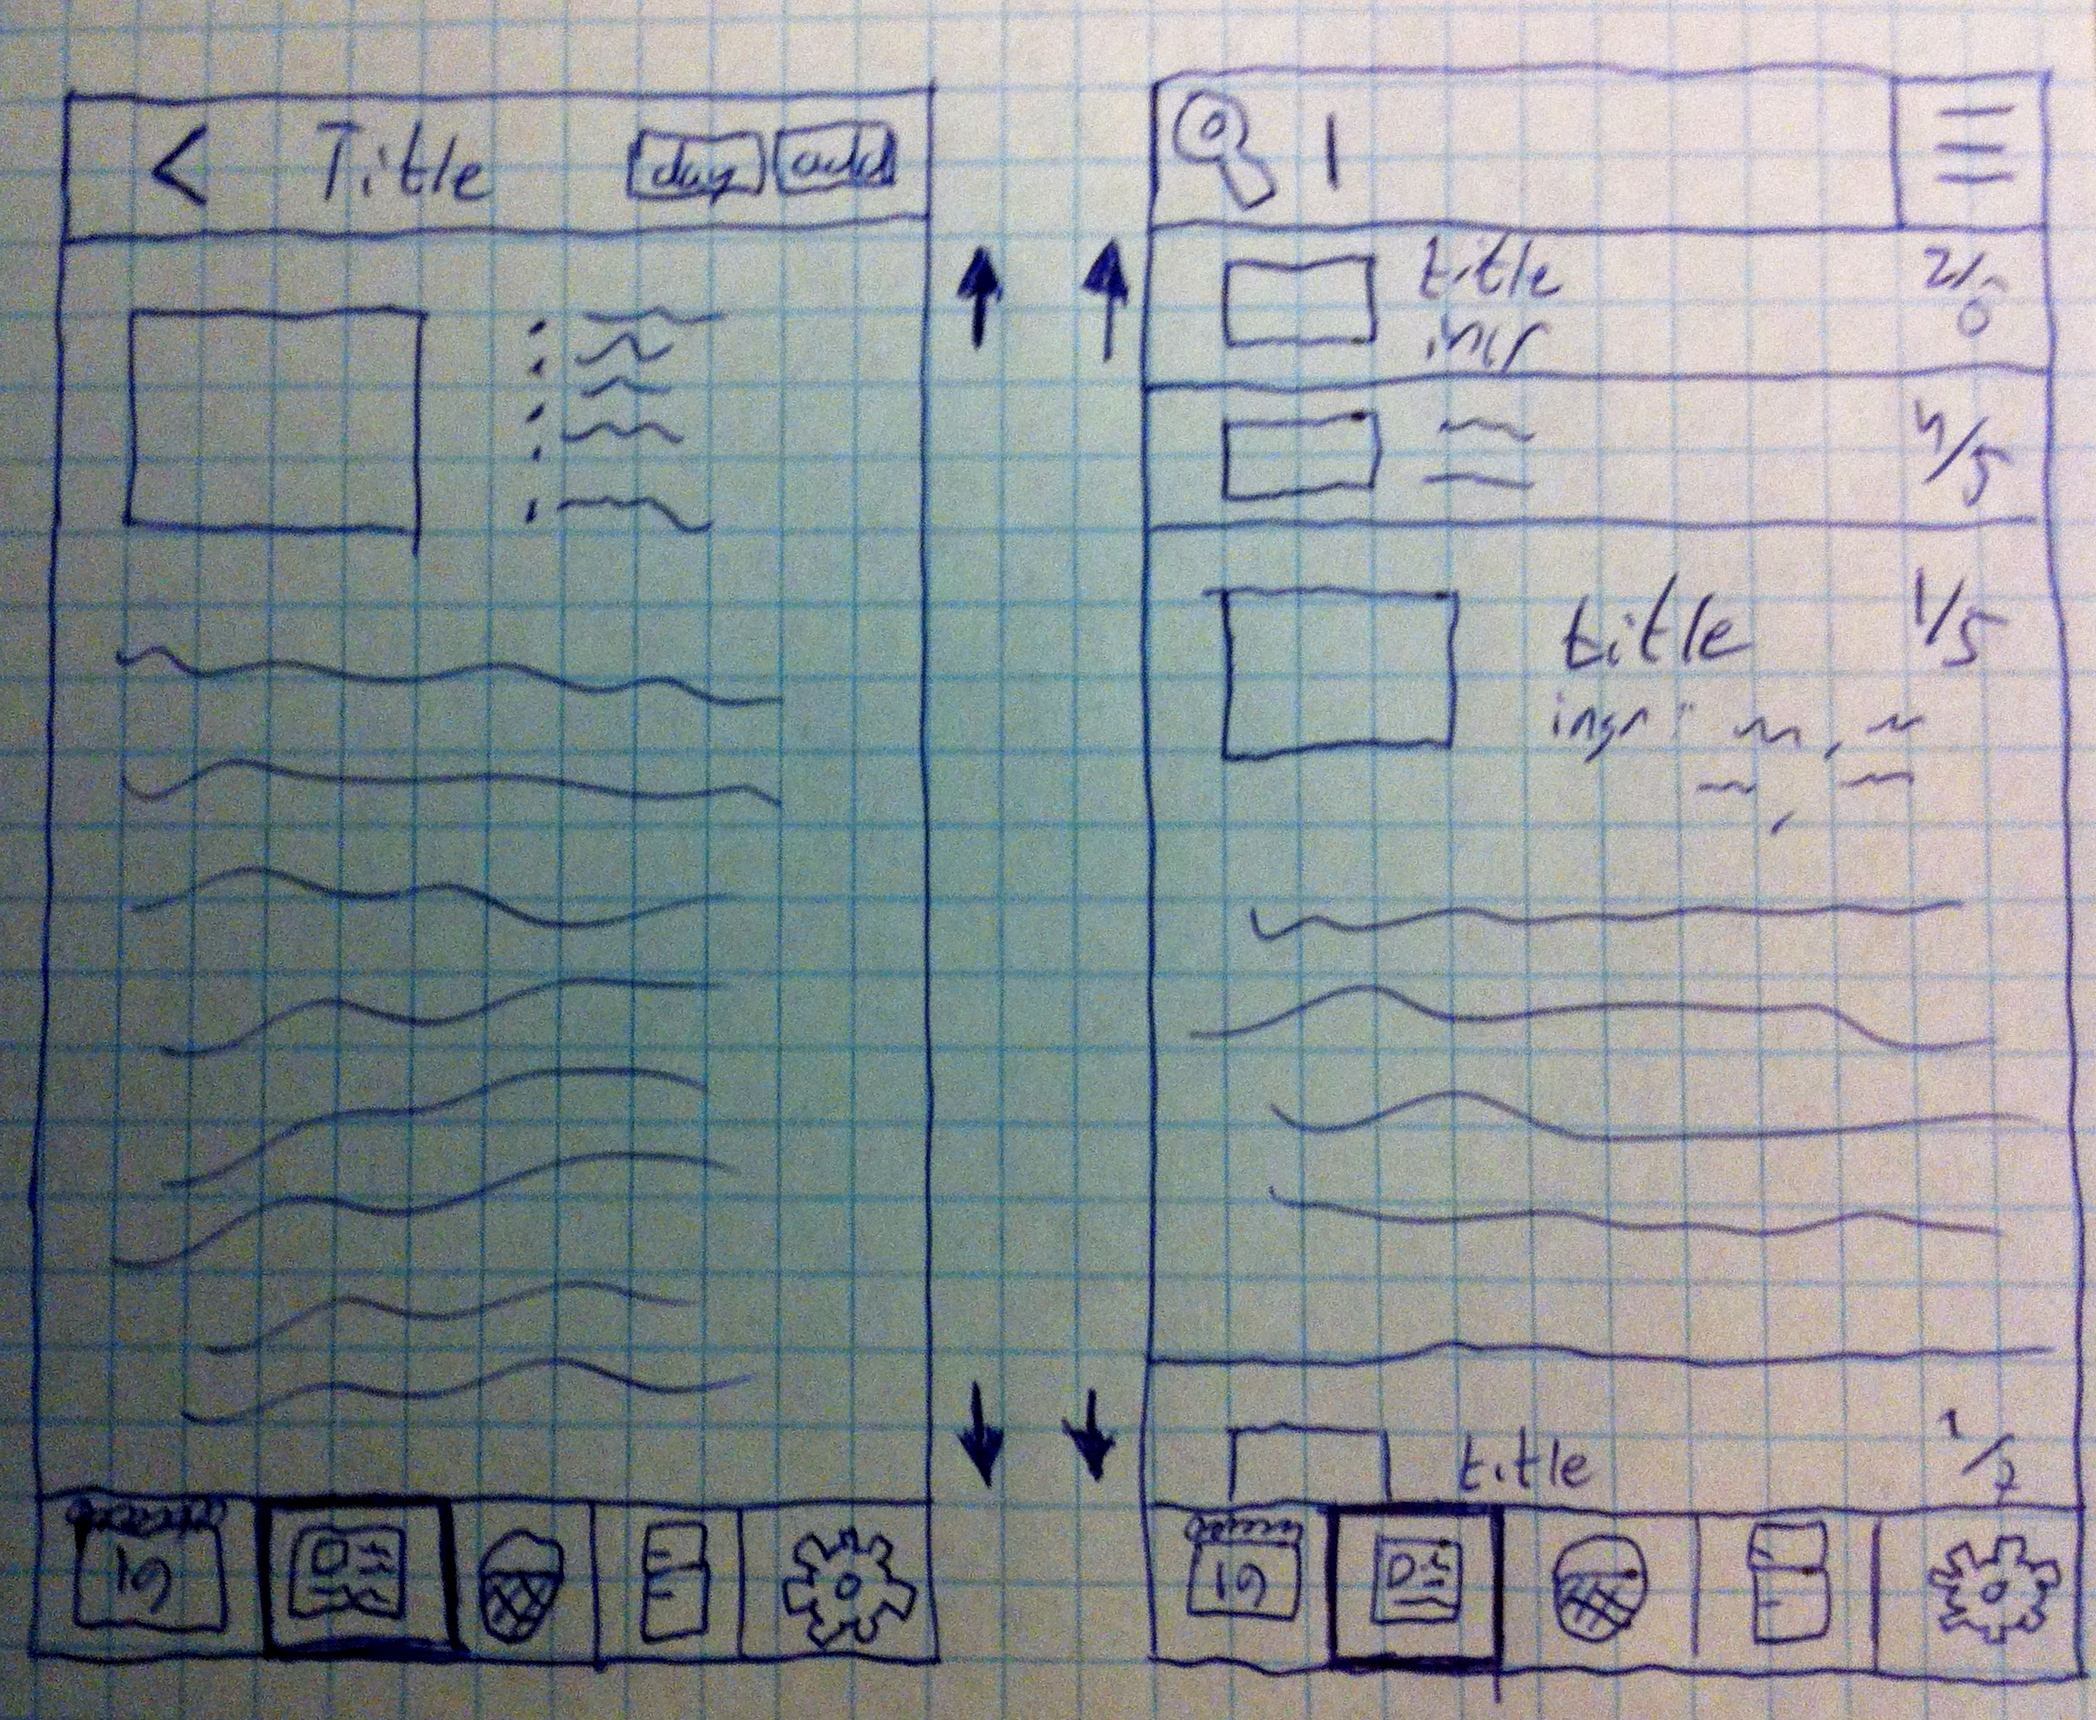
\includegraphics[width=0.5\textwidth]{Grafik/FoodPlanner/FinalRecipeBrowsingSketch2}
    \caption{One of the final sketch of the recipe browsing screen}
    \label{FinalRecipeBrowsingSketch2}
\end{figure}

\subsection{Recipe browsing screen}

The recipes screen is made up of 3 elements, when not counting the general elements of the program. The three elements are:

\begin{itemize}
    \item Search bar
    \item Sort button
    \item List of recipes
\end{itemize}

The search bar is located on the top of the screen, as it is where the users will most likely look for it first, as this is where most search bars in mobile applications, but also websites, is placed. When text is entered into the search bar, the recipes containing the text searched for will be shown in the list of recipes. 

The Sort button offers the user the functionality of sorting the list of recipes by different requirements. It might be by time to cook, by number of ingredients the user already has in the inventory, or by something else. The sort button is located at the right of the search bar, as this was an easy and convenient place to place it. It only consists of an icon showing that you will be able to sort the recipes by clicking the button.

The list of recipes show the recipes that the user can choose from. These are sorted by the sort button as earlier described, or by the search bar which is also earlier described. If there are more recipes available than the screen can hold, the user will be able to swipe in an upwards motion for more recipes to appear at the bottom and the recipes at the top will disappear. In the right side of each recipe it is shown how many of the ingredients needed to make the recipe the user already have; an example is if the user has 4 out of the 10 ingredients needed the right side will show "4/10".

\subsection{Expanded recipe browsing screen}

The expanded recipe screen can be seen in figure \ref{FinalRecipeBrowsingSketch2} on the right. As seen it looks like the recipe browsing screen, but the difference is that this screen show more information about a specific recipe.

When the user has chosen a recipe, the user will be able to click it. By doing to, the recipe will expand, and more information about the recipe will be shown. This will only be the most relevant information, such as ingredients, cooking time, and a picture.

\subsection{Full screen recipe screen}

The full screen recipe screen is the left sketch in figure \ref{FinalRecipeBrowsingSketch2}. This screen gives the full overview of the recipe.

In the left side, a picture of the recipe will be shown if available, and the ingredients will be on the right side of the picture. If there are needed more ingredients that the picture is long, the ingredients will also appear underneath. After the ingredients list is the instructions to make the recipe. If the recipe is longer than the amount of text the screen can hold, the user will be able to scroll through the rest of the recipe using the fingers.

In the top of the screen is a navigation bar. This navigation bar gives the user the ability to do three things:

\begin{itemize}
    \item Go back
    \item Change the amount of people attending the meal
    \item Add the recipe to the meal plan
\end{itemize}

The arrow in the left of the navigation screen indicates a go back function, giving the user the ability to go back to the recipe browsing screen if the user did not want to do anything further with the recipe which is looked upon.

The second element enables the user to change the amount of people attending the meal. THis would change the amount of ingredients needed in the recipe, and would also update the shopping list, so the user would buy the right amount of the ingredients needed.

The last button give the user the functionality to add the recipe being viewed to the meal plan. This would update the shopping list, and add the meal to a specific day chosen by the user.